\chapter{Opis struktury projektu}

\section{Komponenty i Organizacja Systemu}
Projekt Systemu Zarządzania Parkingiem skupia się na zorientowanej obiektowo architekturze, co ułatwia zarządzanie różnymi typami pojazdów i interakcje z parkingiem. Centralnym elementem jest klasa \texttt{Parking}, która zarządza miejscami parkingowymi, a także wprowadzaniem i wyjazdem pojazdów. Klasy pojazdów, takie jak \texttt{Car}, \texttt{Motorcycle} i \texttt{Bus}, dziedziczą z abstrakcyjnej klasy \texttt{Vehicle}, co pozwala na polimorficzne traktowanie różnych typów pojazdów. Poniżej przedstawiono diagram klas, który ilustruje relacje między głównymi komponentami systemu.

\begin{figure}[H]
\centering
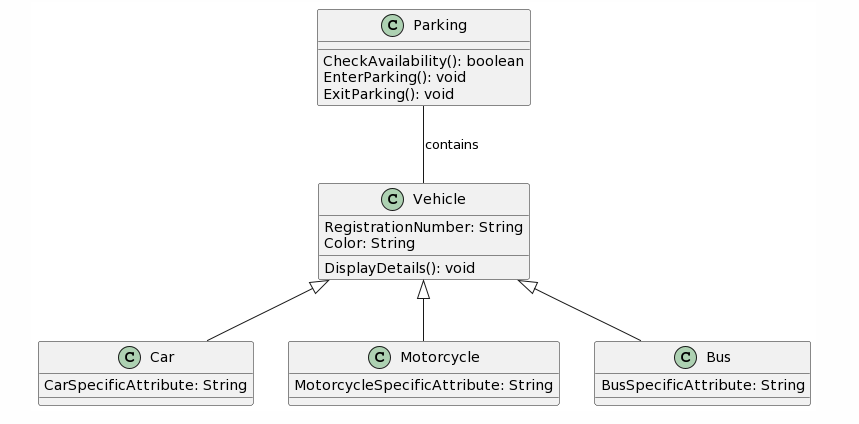
\includegraphics[width=0.75\textwidth]{photos/diagram.png}
\caption{Diagram klas systemu zarządzania parkingiem.}
\end{figure}

Struktura projektu jest zaprojektowana w taki sposób, aby maksymalizować ponowne wykorzystanie kodu i ułatwić rozszerzanie systemu o nowe funkcjonalności.
\clearpage
\section{Opis Techniczny Projektu}

Projekt został zrealizowany w języku C\#, co zapewnia szerokie możliwości w zakresie programowania obiektowego i zarządzania danymi. Do zarządzania projektem i kodem źródłowym wykorzystano środowisko Visual Studio Code z dodatkowymi wtyczkami, takimi jak PlantUML dla generowania diagramów klas UML, oraz Git jako system kontroli wersji.

System jest zaprojektowany z myślą o niskich wymaganiach sprzętowych, co czyni go dostępnym na większości współczesnych komputerów i serwerów. Minimalne wymagania to:
\begin{itemize}
    \item Procesor: 1 GHz lub szybszy.
    \item Pamięć RAM: 512 MB dla klienta, 2 GB dla serwera.
    \item Przestrzeń na dysku: 100 MB.
    \item System operacyjny: Windows 7 lub nowszy, Linux, MacOS.
\end{itemize}

Projekt wykorzystuje mechanizm zarządzania danymi oparty na bazie danych w pliku tekstowym (txt), co pozwala na prostą i efektywną manipulację danymi bez potrzeby korzystania z zewnętrznych systemów DBMS. Taki wybór umożliwia łatwą portowalność i minimalizuje wymagania sprzętowe oraz konfiguracyjne. Struktura plików tekstowych jest zaprojektowana w taki sposób, aby umożliwić szybkie odczytywanie i zapisywanie stanu miejsc parkingowych oraz informacji o pojazdach, co zapewnia wysoką wydajność działania systemu.

\section{Repozytorium i System Kontroli Wersji}

Projekt wykorzystuje system kontroli wersji Git, co umożliwia skuteczne zarządzanie historią zmian kodu źródłowego. Repozytorium kodu znajduje się na platformie GitHub pod adresem:\\ \url{https://github.com/filwalu/ProjektOOP} i będzie dostępne publicznie do dnia 30.09.2024. Bezpieczne\\ połączenie z repozytorium zabezpieczono za pomocą pary kluczy SSH. Poniżej przedstawiono opis\\ użytych poleceń Git:

\begin{enumerate}
    \item \texttt{git init} - inicjalizacja nowego repozytorium Git.
    \item \texttt{git clone [URL]} - klonowanie repozytorium przy użyciu SSH.
    \item \texttt{git add -Av} - dodawanie zmian do kolejki commitów.
    \item \texttt{git status} - sprawdzanie statusu zmian.
    \item \texttt{git commit -m "[wiadomość]"} - commitowanie zmian z opisem.
    \item \texttt{git push} - wysyłanie zmian do zdalnego repozytorium przez SSH.
\end{enumerate}